\documentclass[a4paper,10pt]{article}
\usepackage[utf8]{inputenc}
\usepackage{amsmath}
\usepackage{amsfonts}
\usepackage{amssymb}
\usepackage[german]{babel}
\setlength{\parindent}{0cm}
\usepackage{setspace}
\usepackage{mathpazo}
\usepackage{listings}
\usepackage{graphicx}
\usepackage{wasysym}
\usepackage{booktabs}
\usepackage{verbatim}
\usepackage{ulem}
\usepackage{enumerate}
\usepackage{hyperref}
\usepackage{ulem}
\usepackage{stmaryrd }
\usepackage[a4paper,
left=1.8cm, right=1.8cm,
top=2.0cm, bottom=2.0cm]{geometry}
\usepackage{tabularx}
\usepackage{tikz}
\usetikzlibrary{trees,petri,decorations,arrows,automata,shapes,shadows,positioning,plotmarks}

\newcommand{\rf}{\right\rfloor}
\newcommand{\lf}{\left\lfloor}
\newcommand{\tabspace}{15cm}
\newcommand{\N}{\mathbb{N}}
\newcommand{\Z}{\mathbb{Z}}

\begin{document}
\begin{center}
\Large{Grundlagen der künstlichen Intelligenz: Hausaufgabe 8} \\
\end{center}
\begin{tabbing}
Tom Nick \hspace{2cm}\= - 340528\\
Niklas Gebauer \> - 340942 \\
Leonard Witte \> - 341457 \\
Johannes Herrmann \> - 341091\\
\end{tabbing}

\section*{Aufgabe 1}
    \begin{enumerate}[~~a.)]
	 \item
	 Die erste drei Beispiele werden korrekt klassifiziert (wir gehen in der Tabelle von links nach rechts vor): \\
	 \begin{align*}
	     &sgn(w_{11} \cdot x_1+w_{12} \cdot x_2 - w_{10}) = sgn((-1) + (-1) + 1) = sgn(-1) = -1 = x_1 \oplus x_2 \\
	     &sgn(w_{11} \cdot x_1+w_{12} \cdot x_2 - w_{10}) = sgn(1 + (-1) + 1) = sgn(1) = 1 = x_1 \oplus x_2\\
	     &sgn(w_{11} \cdot x_1+w_{12} \cdot x_2 - w_{10}) = sgn((-1) + 1 + 1) = sgn(1) = 1 = x_1 \oplus x_2
	 \end{align*}
	 Nur Beispiel 4 ändert also die Gewichte:
	 \begin{align*}
        &w_{20} = w_{10} + \lambda y x_0 = -1 + 0.7 \cdot (-1) \cdot (-1) = -0.3 \\
        &w_{21} = w_{11} + \lambda y x_1 = 1 + 0.7 \cdot (-1) \cdot 1 = 0.3\\
        &w_{22} = w_{12} + \lambda y x_2 = 1 + 0.7 \cdot (-1) \cdot 1 = 0.3
	 \end{align*}
	 Nun werden wieder die ersten drei Beispiele korrekt klassifiziert, das 4. allerdings immer noch nicht. Da wir jedes Beispiel nur einmal betrachten sollten, können wir nun aufhören.
	 
	 \item
	 Nein, ein Perzeptron alleine kann die XOR-Funktion nicht erlernen, da die Datenpunkte (Beispiele) nicht linear seperabel sind. Ein einzelnes Perzeptron kann allerdings nur linear separable Datensätze komplett korrekt klassifizieren.
	 
	 \item
    Man kann die Funktion $x_1 \oplus x_2$ umformen:
    \begin{align*}
        x_1 \oplus x_2 \equiv (\lnot x_1 \land x_2) \lor (x_1 \land \lnot x_2)
    \end{align*}
    Das folgende neuronale Netz beschreibt genau diese äquivalente Formel: \\
        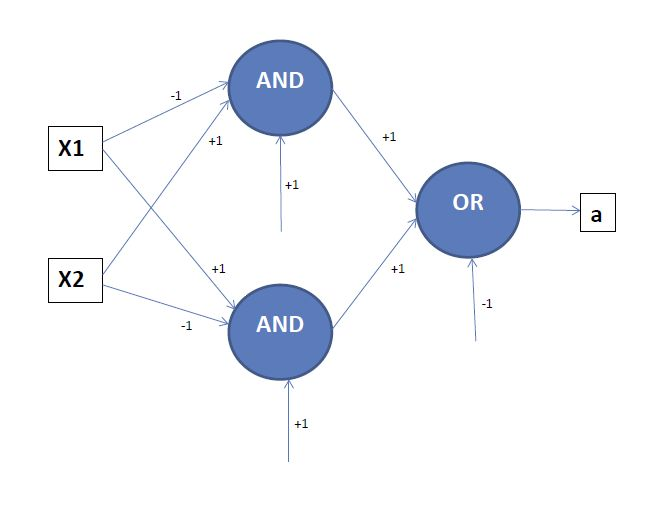
\includegraphics[scale=0.65]{network.jpg} \\
    Die erste Schicht bilden zwei Neuronen, die die UND-Funktion realisieren und jeweils einen der beiden Inputs invertieren. In der zweiten Schicht hingegen haben wir nur ein Neuron, das die beiden Ausgänge der Neuronen der ersten Schicht durch eine ODER-Funktion zum Ausgabewert 'a' verarbeitet: 
	\end{enumerate}

\section*{Aufgabe 2}

\section*{Aufgabe 3}
    \begin{enumerate}[~~a.)]
	 \item
	 Die Ausgabe ist abhängig von p: \\ \\
	 $
	 a(x) = 
	 \begin{cases} 
        1 & ,p > 0,5 \\
        -1 & ,p < 0,5 \\
        x \in [-1;1] & ,p = 0,5
     \end{cases}
     $\\ \\
     Für $p = 0,5$ ist der Wert von $E_1$ immer gleich, daher kann die Funktion dann auf einen beliebigen Wert aus dem Intervall abbilden. Dieser muss natürlich fest gewählt werde.
	 \item
	 Die gesuchte Funktion ist $E_2$. Denn wenn wir ihr Minimum berechnen, indem wir die erste Ableitung gleich Null setzen, sehen wir, dass wir genau die beschriebene Formel für a(x) erhalten:
	 \begin{align*}
	 &E_2' = ( \sum_{i=1}^N |y_i - a(x_i)|^2)' = (p(1-a(x))^2+(1-p)(1+a(x))^2)' = -4p+2a(x)+2 \\
	 &-4p+2a(x)+2 = 0 \Leftrightarrow a(x) = 2p-1
	 \end{align*}
	 
	% TODO: Beweisen, dass es nur genau ein n gibt!
	 \item
	 $p = 0,9$ und $N = 100$ bedeutet wir haben 90 positive und 100 negative Datenpunkte. Für $E_2$ wissen wir, dass das Minimum bei $a(x) = 2p-1$ liegt.\\Also haben wir für unsere Werte ein Minimum bei:\\
	 $2\cdot 0,9 - 1 = 0,8$!\\
	 \\
	 Für $E_3$ bilden wir die Ableitung und setzen gleich Null:
	 \begin{align*}
	  &E_3' = ( \sum_{i=1}^N |y_i - a(x_i)|^3)' = (90(1-a(x))^3+10(1+a(x))^3)' = -240 a(x)^2+600 a(x)-240 \\
	 &-240 a(x)^2+600 a(x)-240 = 0 \Leftrightarrow a(x)_1 = 0,5 \text{ oder } a(x)_2 = 2
	 \end{align*}
	 Da für $a(x)$ nur Werte aus dem Intervall $[-1;1]$ in Frage kommen, liegt unser Minimum der kubischen Fehlerfunktion mit den gegebenen Parametern bei $0,5$.
	 
	\end{enumerate}

\end{document}